\section{research}

Universities are normally structured into disciplines which foster disciplinary research. However, the ubiquity of Informatics in our culture has led to pressures for research that is interdisciplinary. Pressures in favour of such research comes from academics themselves, student interests, external funding sources, and sometimes from university leadership. The 
following subsections discuss the answers obtained for each specific
question.

\subsection{Desirability of interdisciplinary research}

\begin{figure}[h]
\centering
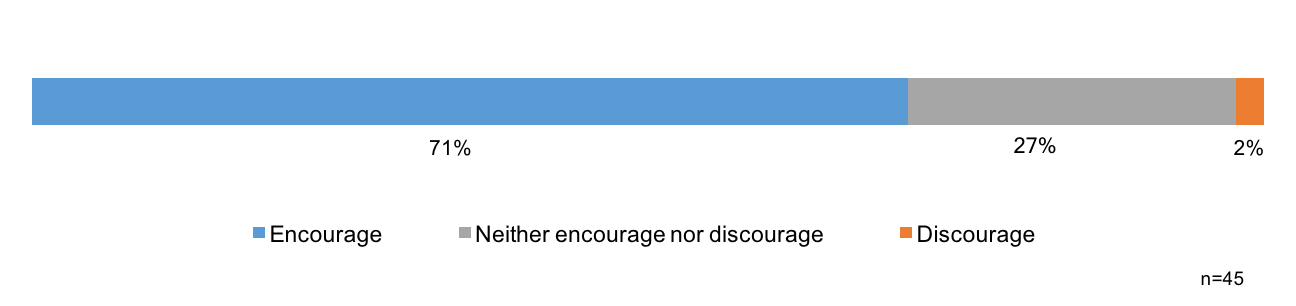
\includegraphics[width = \linewidth]{charts/1a.png}
\caption{What is the University attitude towards Interdisciplinary research?}
\label{sect1:Uattitude}
\end{figure}

The first part of the survey questioned respondents on university attitudes and actions in respect of interdisciplinary research.\footnote{The survey does not differentiate between interdisciplinary work in general and that with an Informatics component. Given who answered the questionnaire, one can assume that Informatics is included} A large majority (71\%) claimed that their university encouraged interdisciplinary research when compared with single discipline research (see Figure~\ref{sect1:Uattitude}). This seems to imply that universities favour interdisciplinary research over single discipline research.  However, several respondents indicated that their encouragement was largely `theoretical' and accompanied by little, if any, funding. Some respondents said that much of the interdisciplinary work at their institution occurred between departments other than Informatics. Only one respondent indicated that their university actually discouraged interdisciplinary research although others mentioned that their departments were judged, usually nationally, against discipline-specific criteria.

\subsection{Department attitude towards Interdisciplinary research}


\begin{figure}[h]
\centering
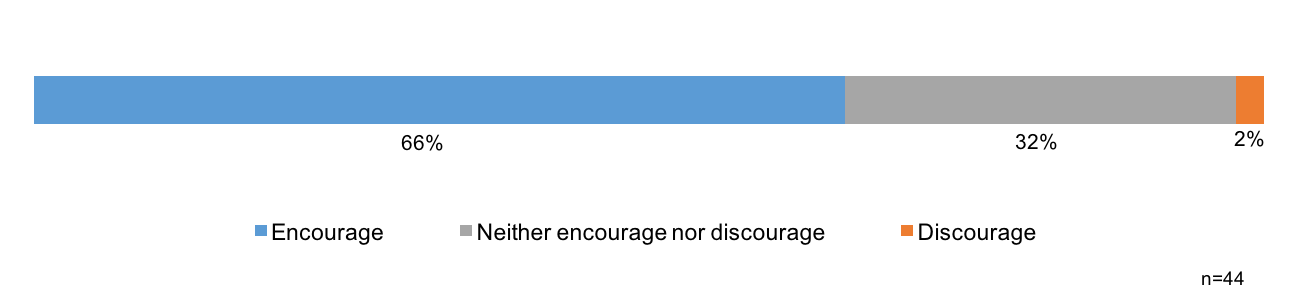
\includegraphics[width = \linewidth]{charts/1b.png}
\caption{What is the Department attitude towards interdisciplinary research?}
\label{sect1:Dattitude}
\end{figure}

With the same question directed at Informatics Departments rather than the whole university (see Figure~\ref{sect1:Dattitude}), two thirds of respondents still claimed that interdisciplinary research was favoured over single discipline topics. However, similar comments are made about encouragement being in principle rather than in practice and about being judged on discipline-specific criteria.

\subsection{University support}

\begin{figure}[h]
\centering
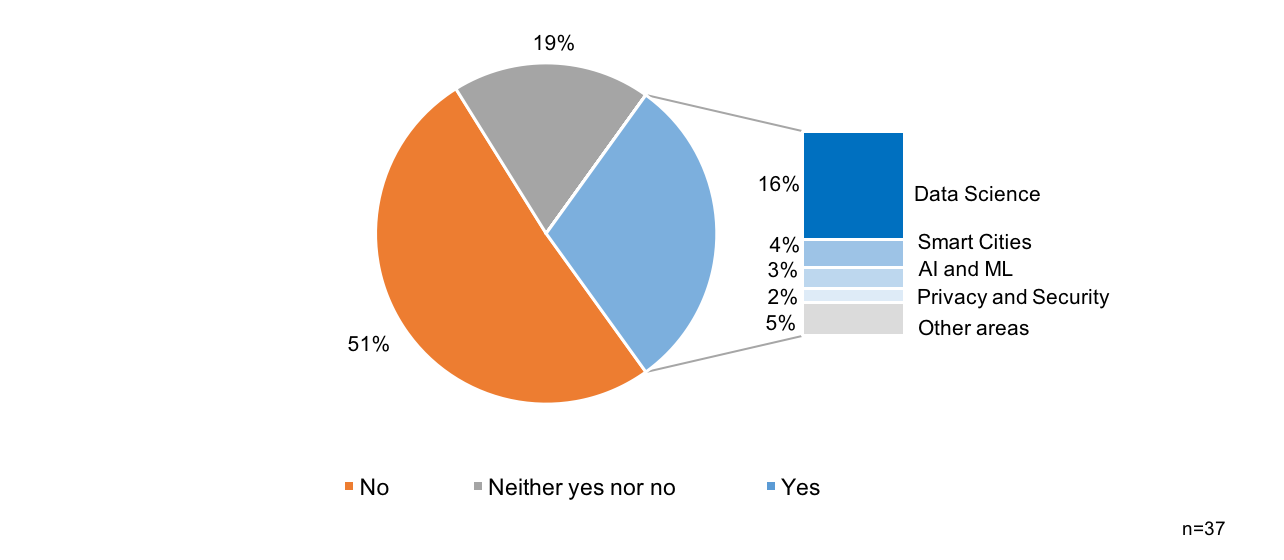
\includegraphics[width = \linewidth]{charts/1c.png}
\caption{Are there interdisciplinary areas of research where your university
could enter but aren't due to lack of university support?}
\label{sect1:support}
\end{figure}

However, just over half (51\%) of the respondents recorded (see Figure~\ref{sect1:support}) that their university supported all areas of interdisciplinary research which required  support. Others (30\%) mentioned a variety of potential informatics areas where university support for interdisciplinary research was lacking. Others talked of the need for strategic planning to direct interdisciplinary efforts or of the need to focus given the wide range of potential opportunities.

\subsection {Additional support}

\begin{figure}[h]
\centering
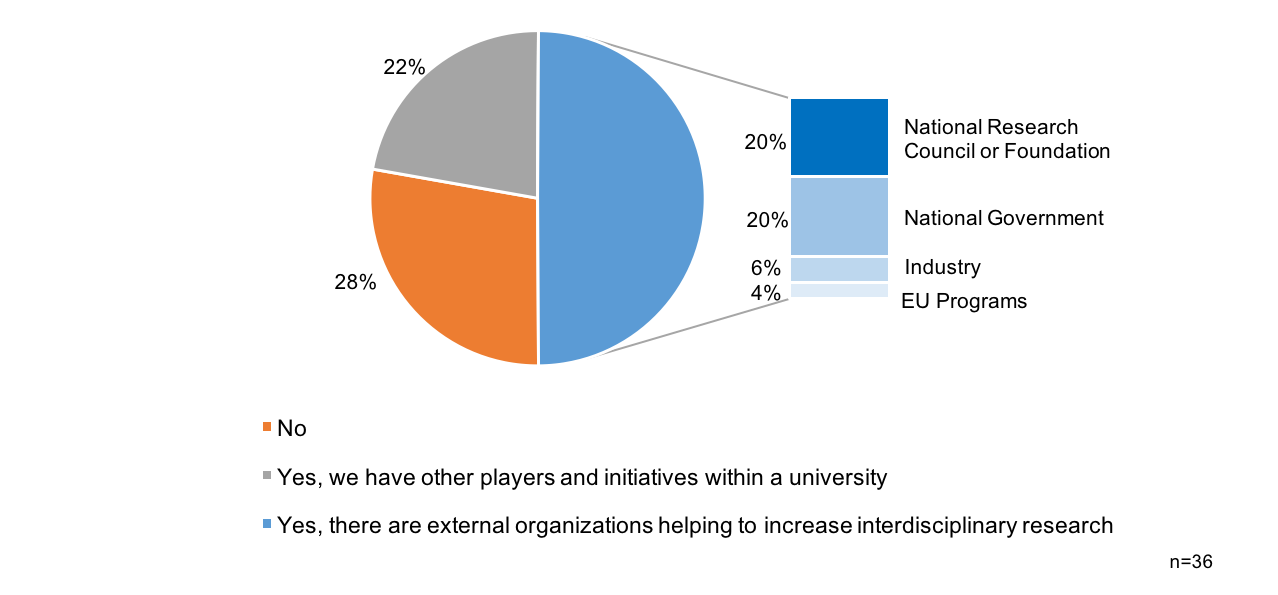
\includegraphics[width = \linewidth]{charts/1d.png}
\caption
{Are there other players who have helped increase the
interdisciplinary research in your university?}
\label{sect1:additional}
\end{figure}

When asked about external support for interdisciplinary research directed towards their university (see Figure~\ref{sect1:additional}), 50\% of the respondents responded positively with 40\% stating that national public funding sources had helped to increase interdisciplinary research. A further 22\% mainly discussed specific formal or informal arrangements between their department and others in their institution.

\subsection{Final thoughts}

Respondents were asked to make some more general comments. Not all respondents were especially supportive of interdisciplinary research per se. It was noted that, because some funding streams demand interdisciplinarity, it is possible that `artificial collaborations' were formed that attracted the funds but did not make good use of the capabilities of the researchers. Frequently interdisciplinary projects are focussed on how information technology can serve the other discipline so the progress made and any breakthroughs that occur advance the other discipline but have no impact on the development of Informatics. One respondent suggested that the excitement and interest in supporting interdisciplinary projects could make it likely that lower quality proposal were accepted (compared with single discipline ones).

Respondents with more positive attitudes towards interdisciplinary research were often nevertheless concerned about its development mainly owing to limited funding, low esteem compared with discipline-specific research or lack of strategic direction.

